\begin{center}
\LARGE
Delprøve uden hjælpemidler 
\end{center}
\stepcounter{section}
%%%%%%%%%%%%%%%%%%%%%%%%%%%%%%%%%%%%%%%%%%%%%%%%%%%%%%%%%%%%%%%%%%%%%%%
%							Ny Opgave!!!!!							%
%%%%%%%%%%%%%%%%%%%%%%%%%%%%%%%%%%%%%%%%%%%%%%%%%%%%%%%%%%%%%%%%%%%%%%%
\begin{opgavetekst}{Opgave 1}
	På \ref{fig:haeldning} ses et hældningsfelt for en differentialligning.
	\begin{figure}[H]
		\centering
		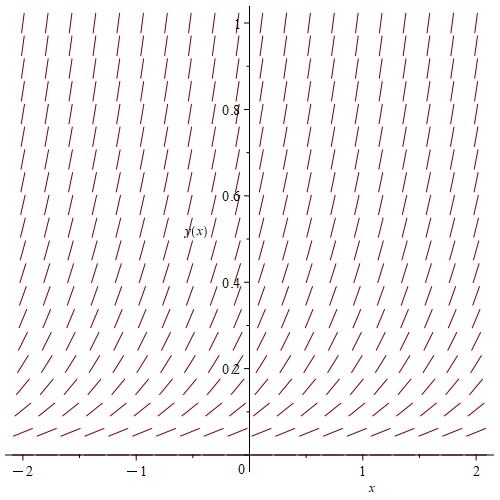
\includegraphics[width=0.5\textwidth]{Billeder/haeldning.png}
		\caption{Hældningsfelt for differentialligning.}
		\label{fig:haeldning}
	\end{figure}
	\phantom{h}
\end{opgavetekst}
	\begin{delopgave}{}{1}
		Afgør, om funktionen $f$ givet ved
		\begin{align*}
			f(x) = e^{-2x}
		\end{align*}
		kan være en partikulær løsning til differentialligningen
	\end{delopgave}
%%%%%%%%%%%%%%%%%%%%%%%%%%%%%%%%%%%%%%%%%%%%%%%%%%%%%%%%%%%%%%%%%%%%%%%
%							Ny Opgave!!!!!							%
%%%%%%%%%%%%%%%%%%%%%%%%%%%%%%%%%%%%%%%%%%%%%%%%%%%%%%%%%%%%%%%%%%%%%%%
\begin{opgavetekst}{Opgave 2}
	En funktion $f:\mathbb{R}^2 \to \mathbb{R}$ er givet ved
	\begin{align*}
		f(x,y) = xy^2-x-y.
	\end{align*}
	\phantom{h}
\end{opgavetekst}
	\begin{delopgave}{}{1}
		Vis, at punkterne 
		\begin{align*}
			&\left(-\frac{1}{2},-1,f\left(-\frac{1}{2},-1\right)\right)\textnormal{ og} 
			&&\left(\frac{1}{2},1,f\left(\frac{1}{2},1\right)\right)
		\end{align*}
		er stationære punkter for $f$. 
	\end{delopgave}
	\begin{delopgave}{}{2}
		Arten af de stationære punkter er ens. Bestem arten af de stationære punkter. 
	\end{delopgave}
%%%%%%%%%%%%%%%%%%%%%%%%%%%%%%%%%%%%%%%%%%%%%%%%%%%%%%%%%%%%%%%%%%%%%%%
%							Ny Opgave!!!!!							%
%%%%%%%%%%%%%%%%%%%%%%%%%%%%%%%%%%%%%%%%%%%%%%%%%%%%%%%%%%%%%%%%%%%%%%%
\begin{opgavetekst}{Opgave 3}
	En kugle $K$ er givet ved ligningen
	\begin{align*}
		K: \ x^2-2x+y^2-4y+z^2+8z=4
	\end{align*}
\end{opgavetekst}
\begin{delopgave}{}{1}
	Afgør, om punktet $(1,2,2)$ ligger på kuglen.
\end{delopgave}
\begin{delopgave}{}{2}
	Bestem centrum og radius for $K$.
\end{delopgave}
%%%%%%%%%%%%%%%%%%%%%%%%%%%%%%%%%%%%%%%%%%%%%%%%%%%%%%%%%%%%%%%%%%%%%%%
%							Ny Opgave!!!!!							%
%%%%%%%%%%%%%%%%%%%%%%%%%%%%%%%%%%%%%%%%%%%%%%%%%%%%%%%%%%%%%%%%%%%%%%%
\begin{opgavetekst}{Opgave 4 }
	En differentialligning er givet ved 
	\begin{align}\label{eq:diffyq}
		y' + \frac{2}{x}y = 3\cos(x^3).
	\end{align}
\end{opgavetekst}
\begin{delopgave}{}{1}
	Vis, at \eqref{eq:diffyq} er en førsteordens lineær differentialligning.
\end{delopgave}
\begin{delopgave}{}{2}
	Bestem en løsning til \eqref{eq:diffyq}, der går gennem punktet $(1,\sin(1))$.
\end{delopgave}
%%%%%%%%%%%%%%%%%%%%%%%%%%%%%%%%%%%%%%%%%%%%%%%%%%%%%%%%%%%%%%%%%%%%%%%
%							Ny Opgave!!!!!							%
%%%%%%%%%%%%%%%%%%%%%%%%%%%%%%%%%%%%%%%%%%%%%%%%%%%%%%%%%%%%%%%%%%%%%%%
\begin{opgavetekst}{Opgave 5}
	På en plan $L$ ligger punktet $(1,4,-5)$. Desuden har planen vektoren $\vv{n}$ givet ved
	\begin{align*}
		\vv{n} = 
		\begin{pmatrix}
			-6 \\ 1/2 \\ 10
		\end{pmatrix}
	\end{align*}
	som normalvektor.
\end{opgavetekst}
\begin{delopgave}{}{1}
	Bestem en ligning for $L$.
\end{delopgave}
%%%%%%%%%%%%%%%%%%%%%%%%%%%%%%%%%%%%%%%%%%%%%%%%%%%%%%%%%%%%%%%%%%%%%%%
%							Ny Opgave!!!!!							%
%%%%%%%%%%%%%%%%%%%%%%%%%%%%%%%%%%%%%%%%%%%%%%%%%%%%%%%%%%%%%%%%%%%%%%%
\begin{opgavetekst}{Opgave 6}
	En differentialligning er repræsenteret grafisk på Fig. \ref{fig:logist}.
	\begin{figure}[H]
		\centering
		\begin{tikzpicture}
			\begin{axis}
				[
				axis lines = center, 
				xmin = -1, xmax = 7,
				ymin = -1, ymax = 4,
				xlabel = {$y$},
				ylabel = {$y'$}, 
				]
				\addplot[thick, color = blue!50, domain = 0:6, samples = 1000] {1/3*x*(6-x)};
				\draw[color = purple, thick, dashed] (axis cs:0,3) to (axis cs: 3,3);
				\draw[color = purple, thick, dashed] (axis cs:3,0) to (axis cs: 3,3);
			\end{axis}
		\end{tikzpicture}
		\caption{Grafisk repræsentation af differentialligning.}
		\label{fig:logist}
	\end{figure}
	\phantom{h}
\end{opgavetekst}
\begin{delopgave}{}{1}
	Bestem den fuldstændige løsning til differentialligningen repræsenteret grafisk på  Fig. \ref{fig:logist}.
\end{delopgave}
%%%%%%%%%%%%%%%%%%%%%%%%%%%%%%%%%%%%%%%%%%%%%%%%%%%%%%%%%%%%%%%%%%%%%%%
%							Ny Opgave!!!!!							%
%%%%%%%%%%%%%%%%%%%%%%%%%%%%%%%%%%%%%%%%%%%%%%%%%%%%%%%%%%%%%%%%%%%%%%%

\newpage
\begin{center}
\LARGE
Delprøve med hjælpemidler 
\end{center}
\stepcounter{section}
%%%%%%%%%%%%%%%%%%%%%%%%%%%%%%%%%%%%%%%%%%%%%%%%%%%%%%%%%%%%%%%%%%%%%%%
%							Ny Opgave!!!!!							%
%%%%%%%%%%%%%%%%%%%%%%%%%%%%%%%%%%%%%%%%%%%%%%%%%%%%%%%%%%%%%%%%%%%%%%%


\begin{opgavetekst}{Opgave 6}
	En differentialligning er givet ved
	\begin{align}\label{eq:logistdiff}
		y' = ay(1.73-y).
	\end{align}
\end{opgavetekst}
\begin{delopgave}{}{1}
	Udnyt, at $y' = 0.0106$, når $y = 0.02$.
\end{delopgave}
\begin{delopgave}{}{2}
	Bestem en partikulær løsning $f$ til \eqref{eq:logistdiff}, der går gennem punktet $(4,0.67)$.
\end{delopgave}
\begin{delopgave}{}{3}
	Bestem tallet $f(11)$.
\end{delopgave}
\newpage
%%%%%%%%%%%%%%%%%%%%%%%%%%%%%%%%%%%%%%%%%%%%%%%%%%%%%%%%%%%%%%%%%%%%%%%
%							Ny Opgave!!!!!							%
%%%%%%%%%%%%%%%%%%%%%%%%%%%%%%%%%%%%%%%%%%%%%%%%%%%%%%%%%%%%%%%%%%%%%%%
\begin{opgavetekst}{Opgave 7}
	\begin{center}
		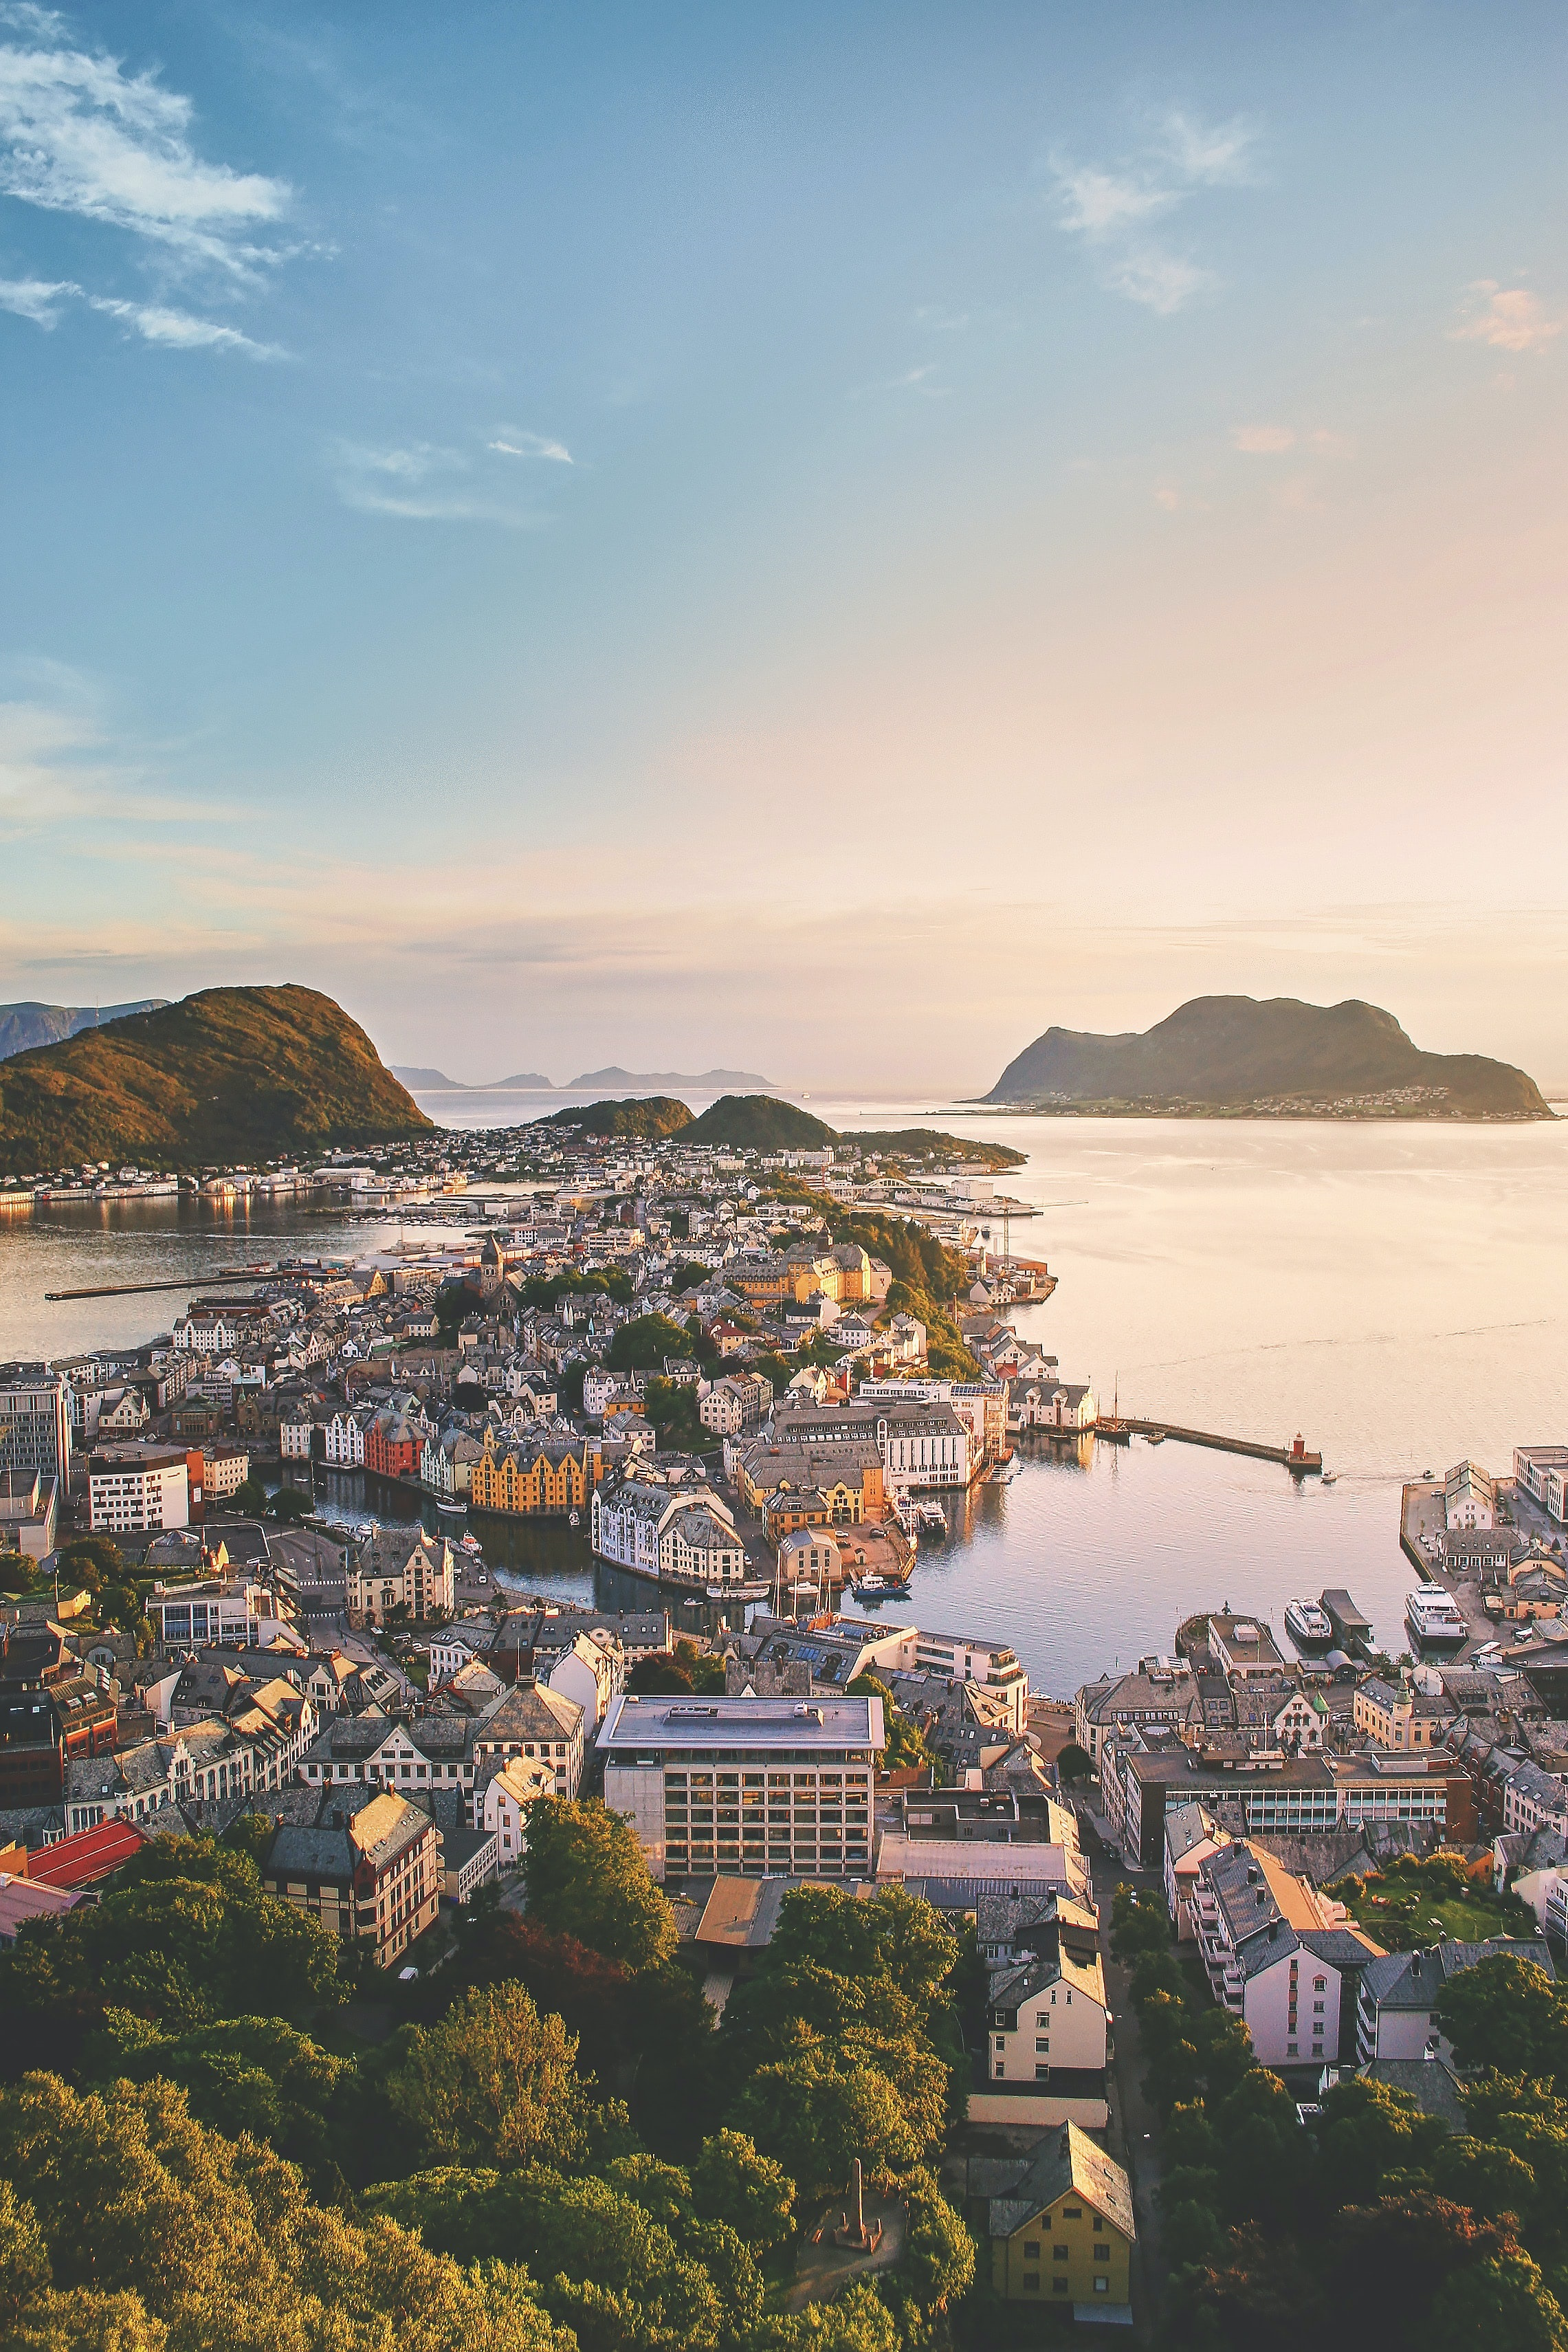
\includegraphics[width=0.4\textwidth]{Billeder/by.jpg}
	\end{center}
 	På Tab. \ref{tab:beboere} ses sammenhængen mellem antallet af beboere i en landsby og antal år efter år 1970.
	\begin{table}[H]
	\centering
	\begin{tabular}{c|c|c|c|c|c|c|c|c}
		År efter år 1970 & $0$ & $5$ & $10$ & $15$ & $20$ & $25$ & $30$&$35$\\
		\hline
		Beboere i tusinde & $1.36$ & $1.99$ & $7.56$ & $11.31$ & $14.73$ & $15.29$ & $15.05$ & $15.15$
	\end{tabular}
	\caption{Antal Beboere i landsby efter år 1970.}
	\label{tab:beboere}
	\end{table}
	\phantom{h}
\end{opgavetekst}
\begin{delopgave}{}{1}
	Lav lineær, eksponentiel og logistisk regression på tallene fra Tab. \ref{tab:beboere}.
\end{delopgave}
\begin{delopgave}{}{2}
	Brug residualerne for de forskellige modeller for at afgøre hvilken af modellerne, der bedst beskriver datasættet. 
\end{delopgave}
\begin{meretekst}
	En analysevirksomhed beslutter sig for at bruge den logistiske model grundet tidligere erfaringer.
\end{meretekst}
\begin{delopgave}{}{3}
	Hvad er det maksimale antal beboere ifølge modellen?
\end{delopgave}
%%%%%%%%%%%%%%%%%%%%%%%%%%%%%%%%%%%%%%%%%%%%%%%%%%%%%%%%%%%%%%%%%%%%%%%
%							Ny Opgave!!!!!							%
%%%%%%%%%%%%%%%%%%%%%%%%%%%%%%%%%%%%%%%%%%%%%%%%%%%%%%%%%%%%%%%%%%%%%%%
\begin{opgavetekst}{Opgave 8}
	\begin{center}
		
\includegraphics[width=0.7\textwidth]{Billeder/tyre.jpg}
	\end{center}
	En importør af bildæk får lovet fra fabrikanten, at der kun vil være fejl på $0.1\%$ af de dæk, han køber. I en sending på 1500 dæk opdager han, at der er fejl på 6 af dækkene, hvilket gør ham 
	mistænksom.
\end{opgavetekst}
\begin{delopgave}{}{1}
	Argumentér for, at antallet af fejl på bildækkene er binomialfordelt og angiv antals- og sandsynlighedsparameteren for fordelingen.
\end{delopgave}
\begin{delopgave}{}{2}
	Opstil en nulhypotese, der kan bruges til at afkræfte mandens mistanke. 
\end{delopgave}
\begin{delopgave}{}{3}
	Lav binomialtest på dataet og afgør, om vi skal forkaste nulhypotesen. 
\end{delopgave}
\newpage
%%%%%%%%%%%%%%%%%%%%%%%%%%%%%%%%%%%%%%%%%%%%%%%%%%%%%%%%%%%%%%%%%%%%%%%
%							Ny Opgave!!!!!							%
%%%%%%%%%%%%%%%%%%%%%%%%%%%%%%%%%%%%%%%%%%%%%%%%%%%%%%%%%%%%%%%%%%%%%%%

\begin{opgavetekst}{Opgave 9}
	\begin{center}
		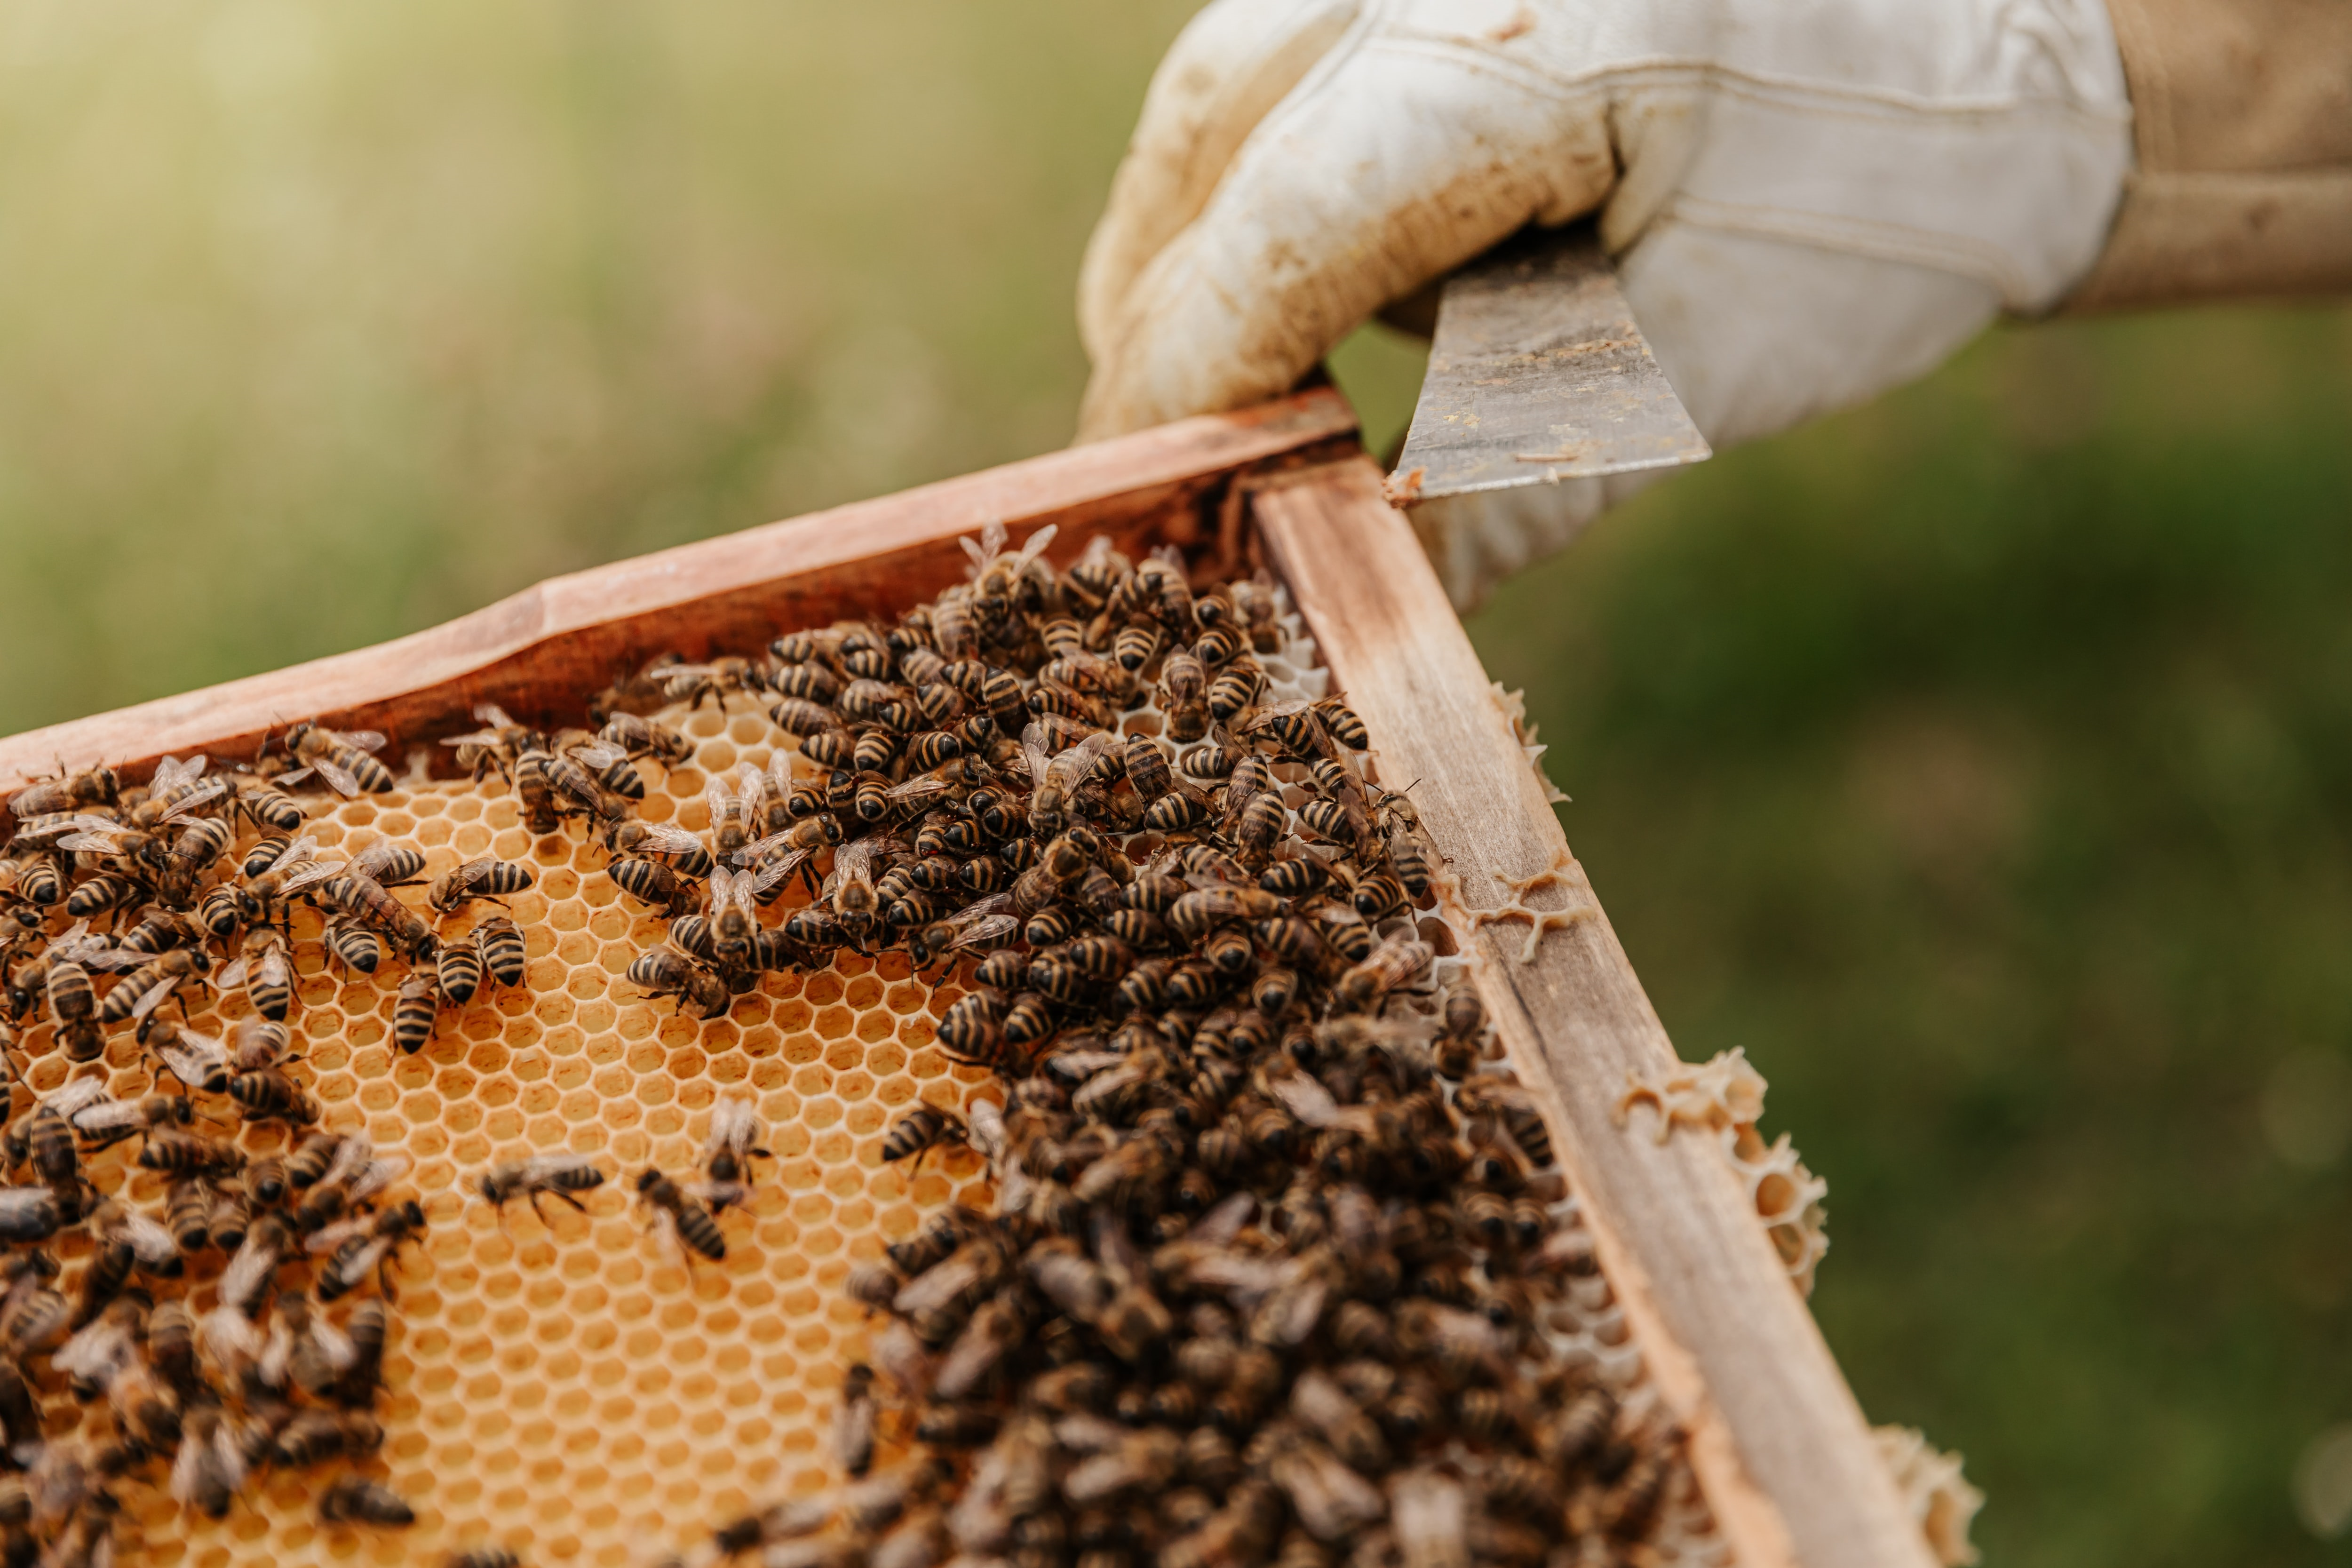
\includegraphics[width=0.7\textwidth]{Billeder/bees.jpg}
	\end{center}
	I en differentialligningsmodel er en bi-bestand vækst $I'$ proportional med antallet af bier $I(t)$ i tusinde efter $t$ uger.
\end{opgavetekst}
\begin{delopgave}{}{1}
	Opstil en differentialligningsmodel, der beskriver væksten af bierne.
\end{delopgave}
\begin{delopgave}{}{2}
	Udnyt, at $I' = 7.2$, når $I = 120$ til at bestemme proportionalitetsfaktoren. 
\end{delopgave}
\begin{delopgave}{}{3}
	Udnyt, at $I(0) = 102.5$ til at bestemme en partikulær løsning til differentialligningen.
\end{delopgave}
\begin{delopgave}{}{4}
	Bestem antallet af bier efter 30 uger. 
\end{delopgave}